\section{Results: ultrasound, capsule endoscopy and chest radiography}\label{sec:multi}

\subsection{Thyroid ultrasound: sonographer calipers}
TN3K images with TNCD labels (3,493 images, 1,210 malignant) carry measurement calipers that a sonographer
places on or around the nodule. Calipers were segmented by an audited rule-based detector (image-level precision
and recall 0.86--0.89). With the E13 protocol unchanged, masking the nodule helps greatly when the calipers lie
outside it (Trap~B: $+0.341$ [$+0.320, +0.363$]) and much less when they lie inside it (Trap~A: $+0.111$
[$+0.097, +0.124$]); the crossover is $+0.230$ [$+0.204, +0.255$] with DINOv2 and $+0.163$ [$+0.132, +0.194$] with
MedSigLIP. After masking, the Trap~A model still relies on the calipers (correlated 0.902 versus reversed 0.400).
With synthetic calipers swept across the nodule boundary (1,663 caliper-free images), masking gains $+0.402$
[$+0.347, +0.458$] at no overlap and $-0.030$ [$-0.079, +0.016$] at full overlap (interaction $+0.432$
[$+0.377, +0.492$]): the entire benefit of masking disappears, without significant harm.

\subsection{Capsule endoscopy: intestinal debris}
SEE-AI frames (erosion 3,550 versus polyp-like 1,931; expert lesion boxes as ROI) with contamination masks from a
patch-token probe trained on 2,160 expert-masked frames (held-out pixel accuracy 0.92, IoU 0.62). Leakage groups
are contiguous blocks of 100 frame numbers plus perceptual-hash duplicates (no video identifiers are published).
Masking helps against out-of-ROI debris ($+0.465$ [$+0.440, +0.490$]) and much less against debris on the lesion
($+0.097$), a crossover of $+0.368$ [$+0.340, +0.397$]. With synthetic debris on the 796 cleanest frames the
reversal appears: $+0.103$ [$+0.060, +0.149$] at no overlap, $-0.102$ [$-0.162, -0.040$] at full overlap
(interaction $+0.205$ [$+0.150, +0.259$]).

\begin{figure*}[t]\centering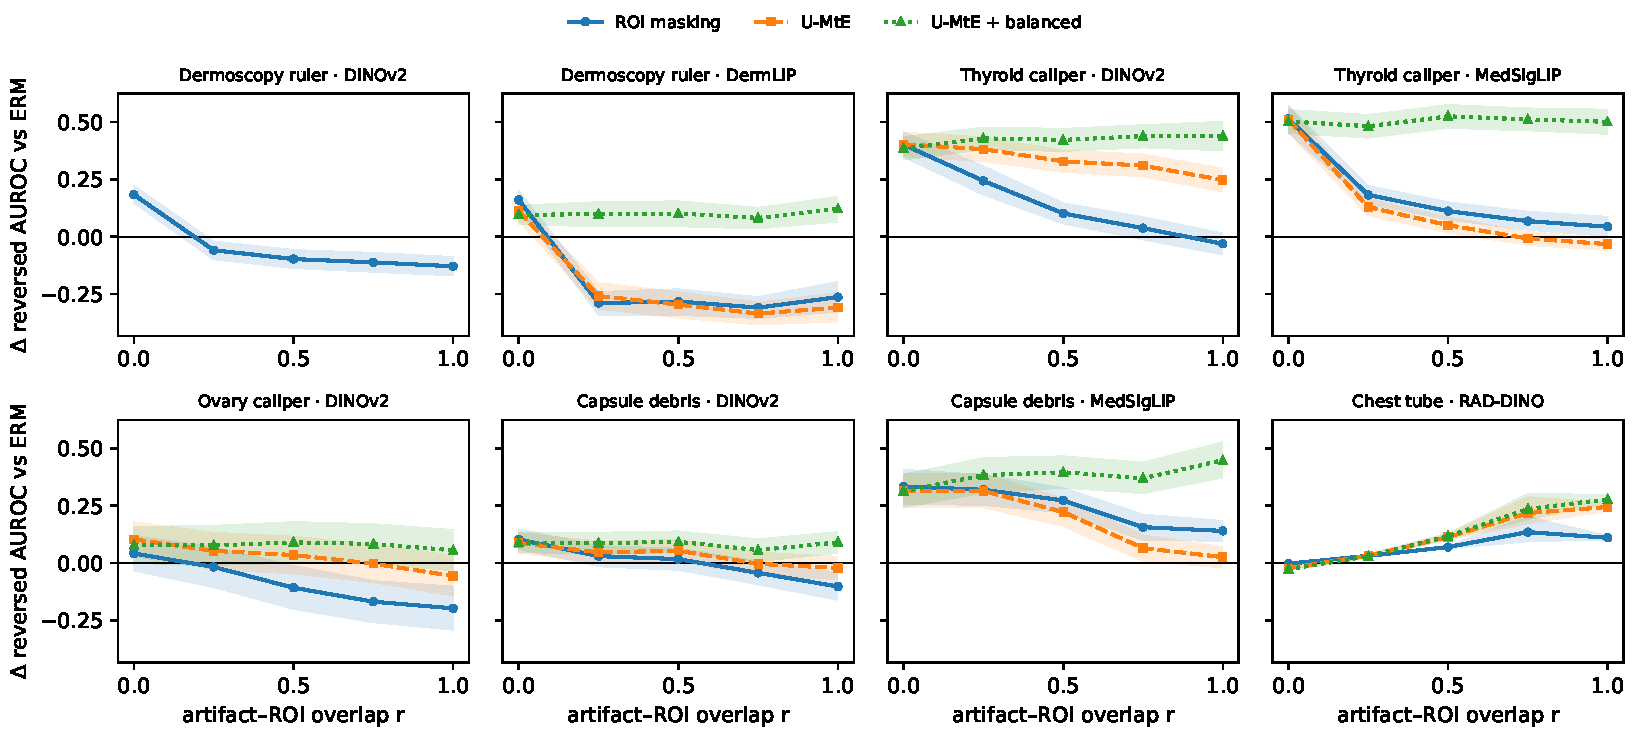
\includegraphics[width=\textwidth]{figures/dose_response.pdf}
\caption{Controlled overlap sweeps: change in reversed-test AUROC versus ERM as the synthetic artifact moves into the
ROI (95\% CIs shaded). ROI masking (blue) declines with overlap in every modality except chest radiography, where the
encoder ignores extra-pulmonary tubes; U-MtE with group balancing (green) is flat. Generated by
\texttt{scripts/make\_figures.py}.}\label{fig:dose}\end{figure*}

\subsection{Chest radiography: a boundary case}
With a synthetic tube swept into the lung fields of NIH pneumothorax radiographs (RAD-DINO), the encoder does not
use an extra-pulmonary tube at all (reversed 0.913 versus clean 0.915 at no overlap), so masking has nothing to
remove; inside the lungs the tube is used (reversed 0.614) and lung masking only partly removes it (0.725). On real
devices (RANZCR-CLiP linked to NIH; central lines and endotracheal tubes) masking helped for both locations. The
location-dependent \emph{harm} of masking is therefore not universal; what is universal in our data is that
masking leaves an in-ROI shortcut largely intact.
